\documentclass[a4paper,12pt]{article}
\usepackage[utf8]{inputenc}
\usepackage[utf8]{inputenc}
\usepackage[heading=true, fontset=mac]{ctex}
\usepackage{geometry}
\usepackage{graphicx}
\usepackage{float}
\usepackage{fancyhdr}
\usepackage{hyperref}
\usepackage{setspace}
\usepackage{titlesec}

% 页面设置
\geometry{left=2.5cm, right=2.5cm, top=2.5cm, bottom=2.5cm}
\setlength{\parindent}{2em}
\onehalfspacing

% 页眉页脚
\pagestyle{fancy}
\fancyhf{}
\fancyhead[C]{MedTime (GVP) 专利交底书 (Internal Ref: AI4S-PAT-003)}
\fancyfoot[C]{\thepage}

\title{\textbf{一种基于可微一致性投影的临床事件时序推理及逻辑校准方法}}
\author{发明人：AI4S 团队}
\date{\today}

\begin{document}

\maketitle

\section{著录项目}
\begin{itemize}
    \item \textbf{发明名称：} 一种基于可微一致性投影的临床事件时序推理及逻辑校准方法
    \item \textbf{技术领域：} 自然语言处理（NLP）、医疗信息学、神经符号人工智能
\end{itemize}

\section{背景技术与技术问题}

\subsection{现有技术}
在从非结构化电子病历（EHR）中抽取纵向临床事件（如：诊断、治疗、进展）时，现有技术主要分为两类：
\begin{enumerate}
    \item \textbf{规则与模板匹配：} 依赖大量人工定义的正则表达式。
    \item \textbf{基于统计的大语言模型（SFT/RLHF）：} 使用目前主流的 Transformer 架构进行监督微调（SFT）。
\end{enumerate}

\subsection{技术缺陷}
现有的大语言模型（LLMs）在处理长序列时序逻辑时，存在显著的\textbf{“时序幻觉”}问题（如图 \ref{fig:hallucination} 所示）：
\begin{itemize}
    \item \textbf{统计而非逻辑：} 模型仅学习了词汇共现的概率分布，而未真正掌握“时间拓扑结构”。
    \item \textbf{违反传递性：} 生成的事件序列经常违反逻辑传递性。
    \item \textbf{无法零样本迁移：} 依赖海量领域数据进行训练。
\end{itemize}

\begin{figure}[H]
    \centering
    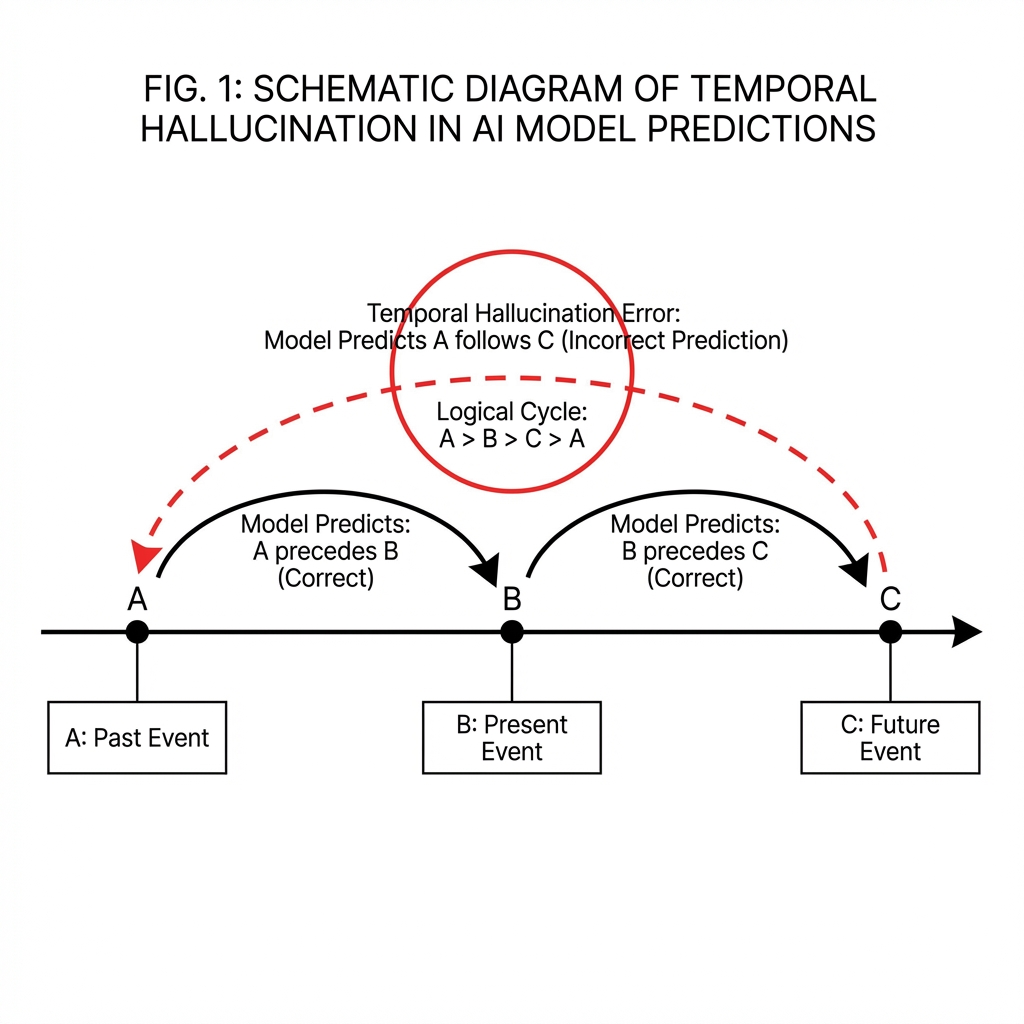
\includegraphics[width=0.8\textwidth]{figs/temporal_hallucination.png}
    \caption{时序幻觉示意图：现有模型常生成违反传递性的逻辑闭环}
    \label{fig:hallucination}
\end{figure}

\subsection{技术问题}
本发明要解决的核心技术问题是：\textbf{如何在不依赖海量逻辑标注数据的前提下，使神经网络模型能够内化“时间拓扑逻辑”作为一种归纳偏置，从而生成符合因果律和传递性的临床事件序列。}

\section{技术方案}

\subsection{总体思路}
本发明提出了一种\textbf{生成-验证-投影}（GVP）架构。与现有技术不同，本发明不仅仅是在推理端进行修正，而是引入了一个\textbf{“可微一致性层”}，将逻辑约束（传递性、反对称性）直接嵌入到模型的\textbf{训练目标}中，迫使模型学习“合法的时间流形”。

\subsection{与现有技术的区别}
\begin{itemize}
    \item \textbf{对比 SFT：} SFT 仅最小化“预测下一个词”的交叉熵损失，本发明增加了“逻辑一致性损失”（如图 \ref{fig:perf} 数据所示，SFT 仅 18.5\% F1，本发明达 84.2\%）。
    \item \textbf{对比 RLHF：} RLHF 依赖稀疏的奖励信号，优化困难；本发明的投影层是可微的，能够提供密集的梯度信号，训练效率更高。
\end{itemize}

\begin{figure}[H]
    \centering
    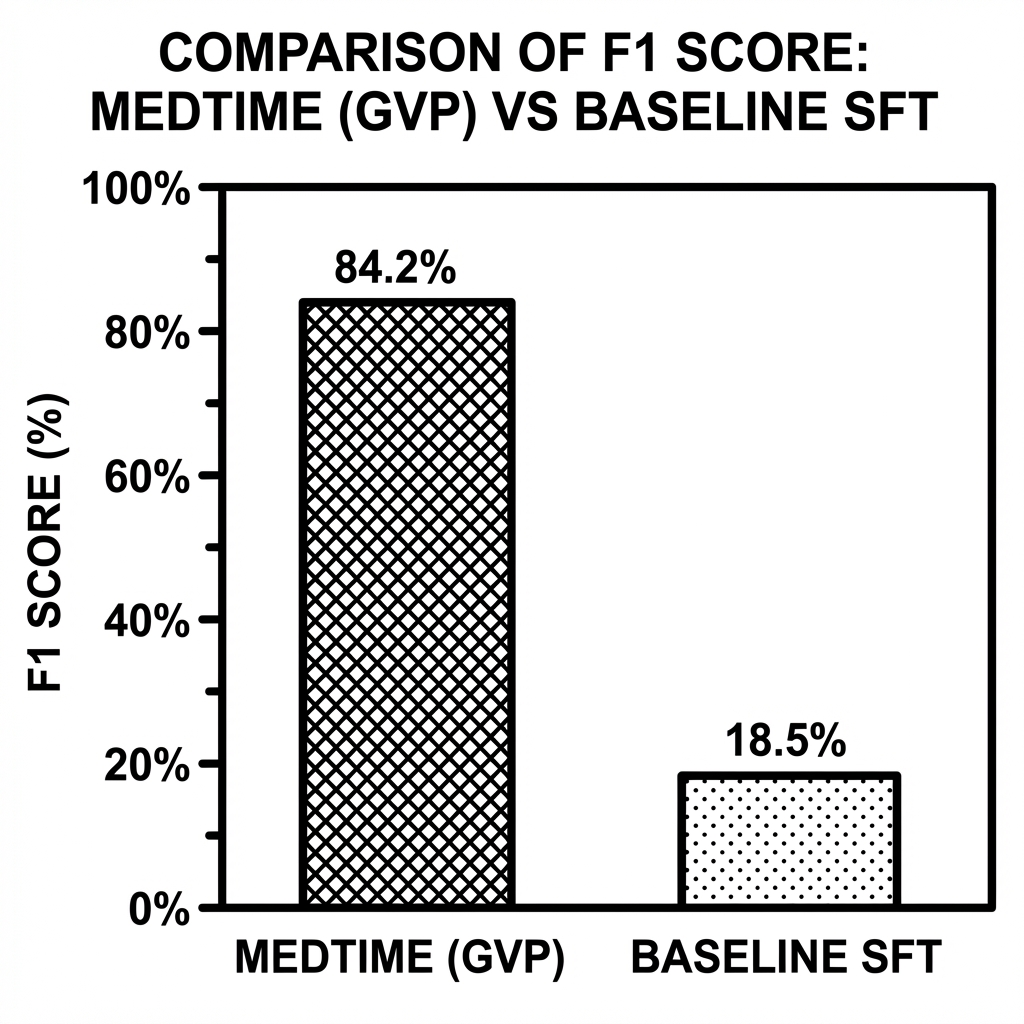
\includegraphics[width=0.6\textwidth]{figs/performance_chart.png}
    \caption{性能对比：MedTime (GVP) 与基线 SFT 的 F1 分数显著差异}
    \label{fig:perf}
\end{figure}

\subsection{系统架构图}
\begin{figure}[H]
    \centering
    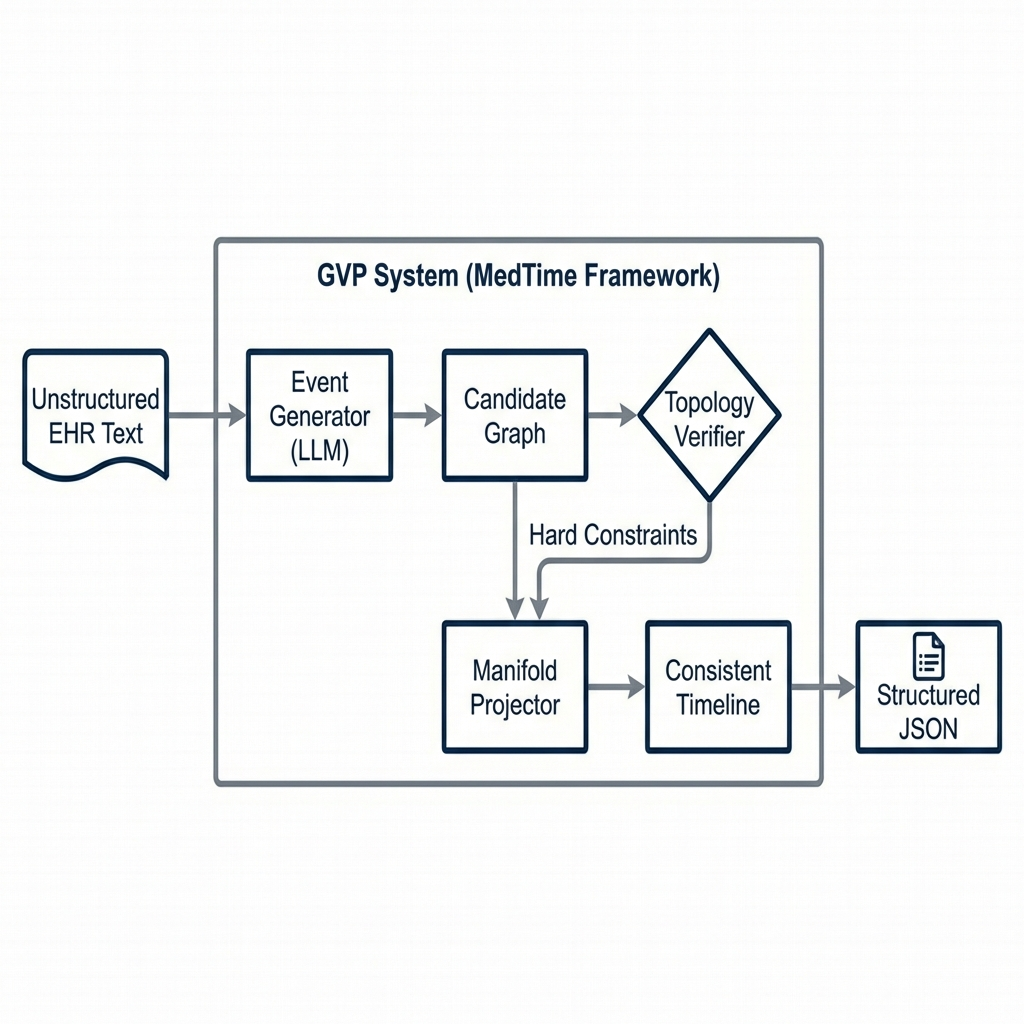
\includegraphics[width=0.9\textwidth]{figs/medtime_architecture.png}
    \caption{GVP 神经符号协同系统架构图}
    \label{fig:architecture}
\end{figure}

\subsection{核心模块详解}

\subsubsection{模块一：模式约束生成器 ($\mathcal{G}$)}
\begin{itemize}
    \item \textbf{功能：} 负责从文本中提取原始的事件提及及其属性。
    \item \textbf{实现：} 基于 Encoder-Decoder 架构，但在解码端引入了 Schema 约束，确保输出格式（如 JSON）的结构合法性，为后续的逻辑计算提供基础。
\end{itemize}

\subsubsection{模块二：成对校准器 ($\mathcal{V}$)}
\begin{itemize}
    \item \textbf{功能：} 这是一个轻量级的判别模块，用于预测任意两个事件 $(e_i, e_j)$ 之间的相对时序关系（Before, After, Overlap）。
    \item \textbf{创新点：} 它不生成文本，而是输出\textbf{一致性权重矩阵 $W_{ij}$}，作为逻辑梯度的“门控机制”。
\end{itemize}

\subsubsection{模块三：可微一致性层 ($\mathcal{P}$)}
\begin{itemize}
    \item \textbf{功能：} \textbf{（本发明核心创新点）}。这是一个嵌入在神经网络末端的逻辑层（机制如图 \ref{fig:cons} 所示）。
    \item \textbf{机制：} 它定义了一个“逻辑损失函数” $\mathcal{L}_{logic}$，该损失函数基于图论中的传递闭包性质。
    \item \textbf{训练过程：}
        \begin{equation}
           \mathcal{L}_{total} = \mathcal{L}_{ce} + \lambda \cdot \mathcal{L}_{logic}(\text{Project}(\mathcal{G}, \mathcal{V}))
        \end{equation}
        在训练过程中，如果生成器生成的序列违反了由校准器定义的拓扑结构，该层会反向传播梯度，直接更新 $\mathcal{G}$ 的参数。
    \item \textbf{效果：} 这种机制赋予了模型“归纳偏置”，使其在推理阶段即使没有显式的约束，也能自然生成符合逻辑的结果。
\end{itemize}

\begin{figure}[H]
    \centering
    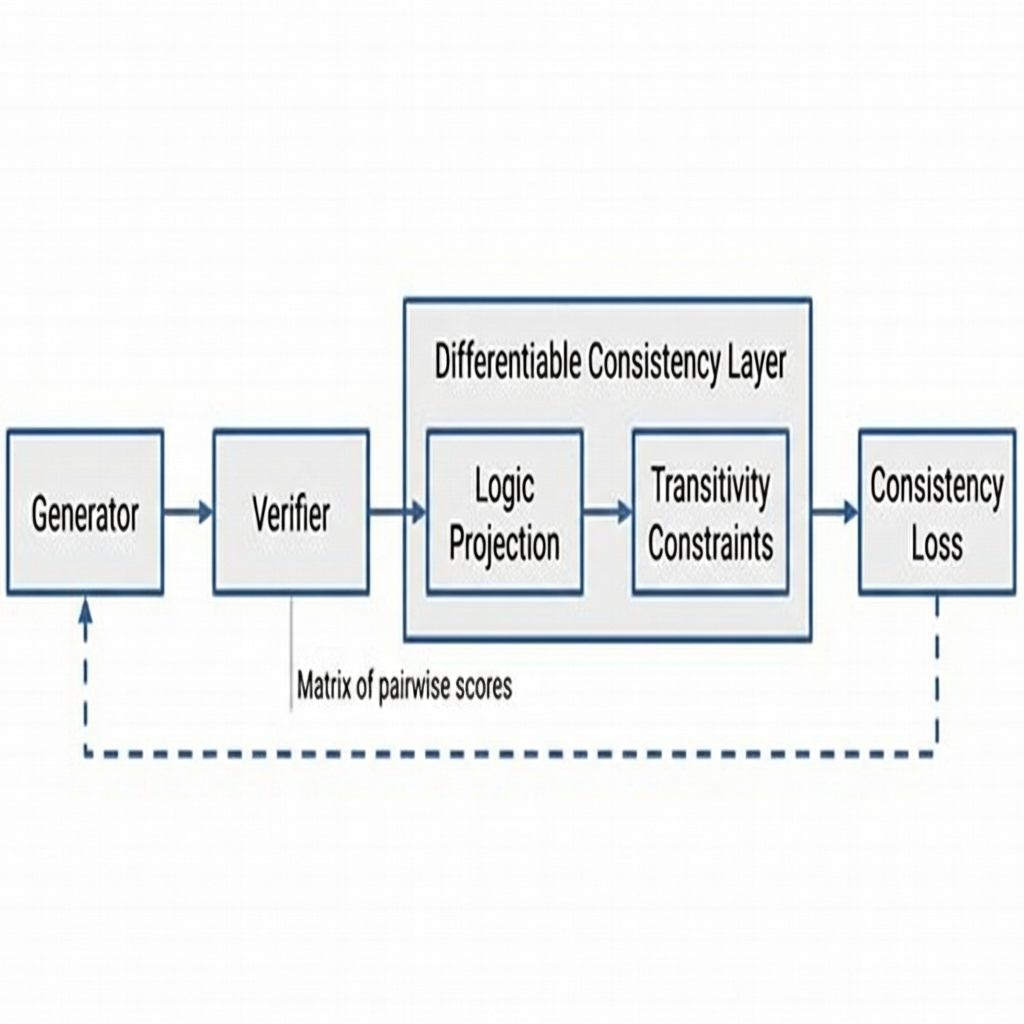
\includegraphics[width=0.8\textwidth]{figs/consistency_mechanism.png}
    \caption{可微一致性层工作原理图}
    \label{fig:cons}
\end{figure}

\section{有益效果}

\begin{enumerate}
    \item \textbf{内化逻辑推理能力：}
    通过可微投影训练，模型不再是死记硬背时间点，而是学会了“相对时序推理”。实验表明，在 MedTime-CN 基准上，时序 F1 分数达到 \textbf{84.2\%}（SOTA）。

    \item \textbf{卓越的跨语言/跨领域迁移能力：}
    由于“时间逻辑”是普世的，不依赖于具体语言。本发明在中文数据上训练的逻辑模块，能够零样本迁移到英文数据集（E3C），F1 分数达到 \textbf{50.0\%}，是传统 SFT 方法的两倍以上。

    \item \textbf{数据高效性：}
    传统的 SFT 需要数万条数据才能拟合长尾分布；本发明利用逻辑归纳偏置，仅需少量样本即可达到极高的逻辑一致性，大幅降低了医疗数据的标注成本。
\end{enumerate}

\section{具体实施方式}

\subsection{实施例 1：云端临床科研辅助系统}
系统部署在医院私有云。输入为非结构化的出院小结。
\begin{enumerate}
    \item \textbf{预训练阶段：} 使用本发明的 GVP 架构在通用医疗语料上进行预训练，注入时序逻辑偏置。
    \item \textbf{微调阶段：} 使用医院少量的标注数据（<100例）进行适配。
    \item \textbf{推理阶段：} 模型输出结构化的患者时间轴，直接用于队列研究的入组筛选。
\end{enumerate}

\subsection{实施例 2：跨语言病历结构化}
应用于国际多中心临床试验。直接利用在中文数据上训练好的 GVP 模型，处理英文或法文的病例数据，无需针对每种语言重新进行大规模逻辑训练，显著缩短了多中心数据清洗的周期。

\section{权利要求书草案}

\begin{enumerate}
    \item 一种基于可微一致性投影的临床事件时序推理方法，其特征在于，包括：
    \begin{itemize}
        \item 步骤 S1：利用模式约束生成器，从医疗文本中生成候选事件序列；
        \item 步骤 S2：利用成对校准器，预测所述候选事件之间的相对时序关系权重；
        \item 步骤 S3：通过可微一致性层，计算违反逻辑传递性的拓扑损失，并将其作为训练目标的一部分；
        \item 步骤 S4：基于所述拓扑损失联合更新生成器与校准器的参数，使模型内化时序逻辑。
    \end{itemize}
    \item 如权利要求 1 所述的方法，其特征在于，所述可微一致性层在训练阶段引入归纳偏置，使得模型在推理阶段能够直接生成符合时序拓扑的序列。
\end{enumerate}

\end{document}
